% Chapter: Requirements spec.

This chapter summarizes and further explains the official assignment of the
project.

\section{Functional Requirements}

This section contains lists of functional requirements split into mandatory
and optional groups.

\subsection{Mandatory Functional Requirements}

This section contains a list of features that must be implemented in the final
solution.

\begin{itemize}
	\item The system recognizes entities in a document and determines their type.
	\item The system assigns recognized entities to objects from the database.
	\item The user will be able to edit recognized entities (add an entity,
	remove an entity, change the type of of an entity, change the range of an
	entity).
	\item The user will be able to edit the assignments of objects to entities.
	\item The user will be able to mark relations between objects.
	\item The user will be able to add types of entities (respectively objects)
	and relations\footnote{For more details see Section \ref{ssec:AddingTypes}}.
	\item The system will continuously learn to recognize entities and to assign
	objects to entities from processed documents confirmed by users.
	\item The user will be able to merge objects saved in the database.
	\item The user will be able to browse objects and relations between them
	stored in the database as lists and as graphs.
	\item The user will be able to use to browse the database these kinds of 
	search:
	\begin{itemize}
		\item a full text search in documents,
		\item a searching for objects or relations by types,
		\item a searching for objects by their aliases,
		\item and combinations of these methods.
	\end{itemize}
	\item The user will be able to suspend ongoing work on the currently
	processed document.
	\item The interrupted work will be stored locally, the processed report will
	be stored in the database after complete  completion work on the document.
	\item The database must log (revise) all performed changes.
\end{itemize}

\subsection{Optional Functional Requirements}

This section contains requirements that are not necessary, but could really
enhance the project's usability if implemented.

\begin{itemize}
	\item The user will be able to cancel a merging of objects followed by
	a semi-automatic assignment of object occurrences, that were recognized
	while they were merged, to divided objects.
	\item The system will recognize relations between objects in a document
	based on relations that users marked before in other documents.
	\begin{itemize}
		\item The user will be able to edit recognized relations between objects
		in the document.
	\end{itemize}
	\item The user will be able to browse the database by more complex kinds of
	search methods:
	\begin{itemize}
		\item a search of connection between objects,
		\item a search of relations by anchors in documents.
	\end{itemize}
\end{itemize}

\section{Non-functional Requirements}

This section contains a list of non-functional requirements, i.e. requirements
not related to functional features demanding specific behavior or functionality.

\begin{itemize}
	\item The system must support a parallel connection of more users.
	\item The system must be able to recover from a crash of server or client.
	\item The system must be connectible with other systems.
	\item The system must reasonably handle an unavailability of the server.
	\item The updating of auto-recognition, learning from new documents,  may
	take a longer time, the system should use the old model during the learning.
	\item The system must be usable without an Internet connection, e.g. in
	a closed intranet.
\end{itemize}

\section{Basic Assumptions}

This section contains a list of basic assumptions that limit the scope of the
project.

\begin{itemize}
	\item Entities are contiguous and not overlap in a document.
	\item An user won't be able to edit a data stored in a database. The only form
	of update will be insertion of a new document and its annotations.
	\item A parallel annotation of a document won't be supported.
	\item The system won't solve an authentization and  an authorization of users.
	\item The system won't solve a backup.
\end{itemize}

\section{Explanations}

\comment[Adam]{Ondrej}{explain main window mockup and that more things can be
done simultaneously}
\comment{Adam}{This needs some title probably, but what?}

Due to the complexity of the tasks required from users, it is necessary to allow
the users to browse the database while they are processing a report, so they
can assign right objects to recognized entities. This can be realized by
embedding inner windows into the main application window or by creating
independent system outer stages (see Figure \ref{fig:MockupMainWindow}).
Then multiple tasks can be performed simultaneously. Implementing both
``inner windows'' and ``outer stages'' approaches and letting the users choose can
significantly improve the user experience.

\begin{figure}[!htb]
        \centering
        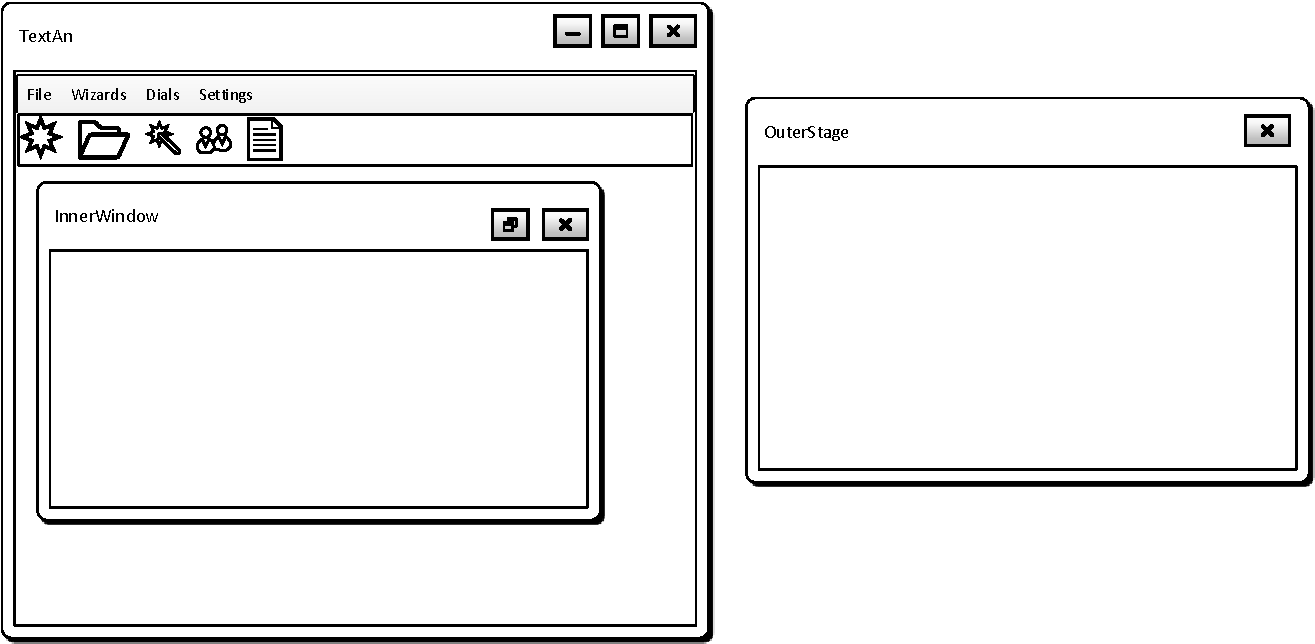
\includegraphics[width=\textwidth]{Images/MockupMainWindow}
        \caption{Mockup screen of the main window.}
        \label{fig:MockupMainWindow}
\end{figure}

\section{Use Case}

The Figure \ref{fig:UseCase} provides a basic overview of interaction within
\textan{} system. There are three expected actors included: a user, an
administrator and an external system. The user represents a human that interacts
with the system through \textan{} client. On the contrary, the other system
represents systems that interacts with \textan{} server over its web API. The
administrator is the person that deploys and configures the system, both the
client and the server.

\begin{figure}[!htb]
        \centering
        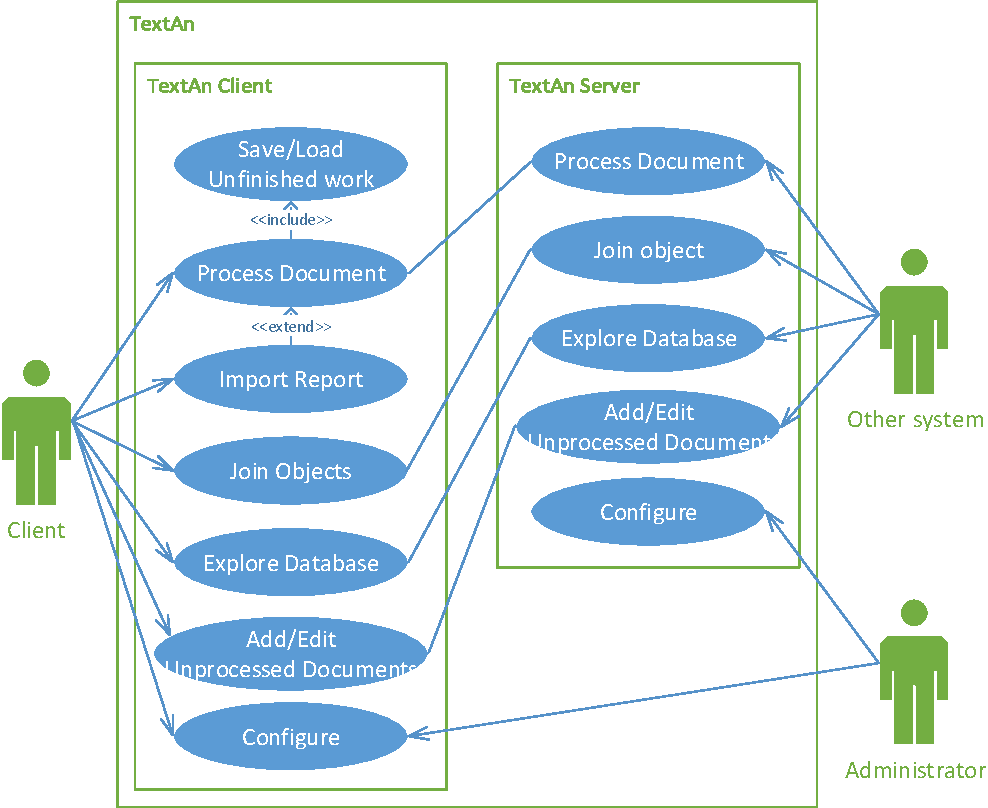
\includegraphics[width=(0.9\textwidth)]{Images/UseCase}
        \caption{Use case of the system.}
        \label{fig:UseCase}
\end{figure}

